\documentclass{article}
\usepackage[utf8]{inputenc}
\usepackage[english]{babel}
\usepackage[document]{ragged2e}
\usepackage[a4paper, total={7in, 9in}]{geometry}
\usepackage{graphicx}
\usepackage{float}
\usepackage{subfigure}
\usepackage{multicol}
\usepackage{comment}

\title{\textbf{CSE520S Project Proposal}\\a wearable radar obstacle-avoid detector}
\author{Bingxin Liu Guohao Pu Hao Liu}
\date{February 2021}

\begin{document}
    \begin{titlepage}
        \maketitle
    \end{titlepage}


    \section{Team Members}
        \begin{flushleft}
            Bingxin Liu, Guohao Pu, Hao Liu\\
        \end{flushleft}
    \section{Project Description}
        \subsection{Motivation}
        Nowadays, human society is developing rapidly while the demand of blind people has merely been noticed. 
        Since there is a few of device designed for the travel convenience of blind people, we plan to meet this demand.  
        
        \subsection{Overview}
        In this project, we plan to develope a wearable obstacle-avoid detector, which is a detective device for blind people. It can detect the existence and distance of obstacles, and then translate those signals into vibration signal.  Blind people can get notice and "feeling" of these obstacles. The distance from the people and obstacles will be translated as the vibration frequencty. If the obstacle is far away from the one who wear the device, the frequency of the vibration is slow. And the frequency will increase  as the one getting closer to these obstacle. Besides, the device has the ability of recording the GPS location of the people who wear it and send it to his guardians, which allows guardians to track the location real time.

        \subsection{System Pieces}
        Basically, our system is aggregated by several sensors and motors, a Raspberry Pi, a GPS module, and the service provided by AWS. Like the figure1 showed, a distance sensor and a vibration motor will be a group. The Raspberry Pi will convert the distance value gathered by distance sensor into frequency value, and send it to vibration motor. A group of those small devices will notice the blinds with information from one specific direction. Therefore, as the number of group increased, the "feeling" will have more and more precise granularity. In our project, we plan to use four or eight gourps of devices due to our limited abilities and budgets.\\
        Furthermore, we will attach an GPS module into our Raspberry Pi, which allows us make use of services supported by AWS IoT. Therefore, we can send neccessary information, like position coordinate, to guardians' devices.\\
        We may also add some other features, in case we have some extra time at the end of this semester.
    
    \begin{multicols}{2}
    \section{Division of Work}
        \textbf{Bingxin} will be responsible for aggregating hardware and develope parts of the software of communicating with hardware.\\
        \textbf{Guohao} will mainly implement parts of software of gathering and sending information to the cloud.\\
        \textbf{Hao} will in charge of designing algorithm to process signals and analysis.

    \section{Equipment}
        \begin{itemize}
            \item a Raspberry Pi
            \item 4 or 8 * distance sensors
            \item 4 or 8 * vibration motors
            \item a GPS module
        \end{itemize}

    \begin{figure}[H]
        \centering
        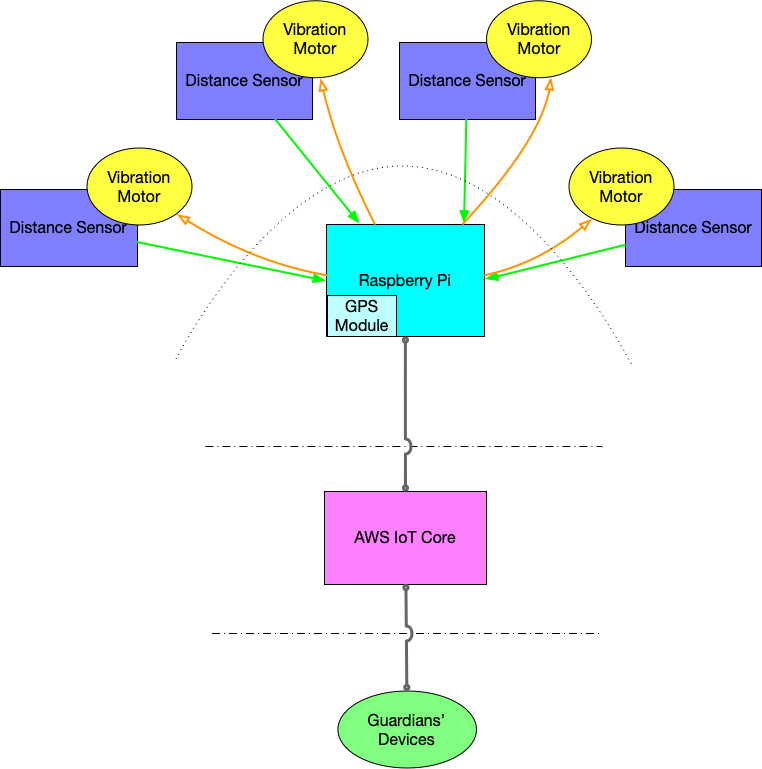
\includegraphics[width=0.4\textwidth]{cse520s_proposal_fig1.jpg}
        \caption{System Design}
    \end{figure}
    \end{multicols}
\end{document}